	% Welcome! This is the unofficial University of Udine beamer template.

% We defined four theme colors: UniBrown, UniBlue, UniGold
% and UniOrange. For example, to write some uniud-brownish
% text, just use: \textcolor{UniBrown}{Hello!}

\documentclass[usenames,dvipsnames]{beamer}
\usepackage[utf8]{inputenc}
\usepackage{verbatim}
\usetheme{uniud}
%\bibliography{bib}
%%% Bibliography
%\usepackage[style=authoryear,backend=biber]{biblatex}
%\addbibresource{bib.bib}
\usepackage{tikz}
\usetikzlibrary{patterns,snakes}
%\DeclareNameAlias{author}{first-last}

%%% Suppress biblatex annoying warning
\usepackage{silence}
\WarningFilter{biblatex}{Patching footnotes failed}

%%% Some useful commands
% pdf-friendly newline in links
\newcommand{\pdfnewline}{\texorpdfstring{\newline}{ }} 
% Fill the vertical space in a slide (to put text at the bottom)
\newcommand{\framefill}{\vskip0pt plus 1filll}
\newcommand{\bigCI}{\mathrel{\text{\scalebox{1.07}{$\perp\mkern-10mu\perp$}}}}
\newcommand\asto{\mathrel{\stackrel{\makebox[0pt]{\mbox{\normalfont\tiny a.s.}}}{\to}}}


\title[Blind Separation of Nonlinear Mixtures]{‌\vspace{0.5cm}\\
Blind Separation of Nonlinear Mixtures of Stochastic Processes}
\author[Behrad Moniri]{
  Behrad Moniri
  \pdfnewline
  \texttt{bemoniri@ee.sharif.edu}
  \pdfnewline\pdfnewline
    \textbf{Advisor}:\\ Prof. Massoud Babaie-Zadeh
}
\institute{\small{EE Department, Sharif University of Technology}}
\date{}
\begin{document}

\begin{frame}
\titlepage
\end{frame}

\begin{frame}{Outline}
\tableofcontents
\end{frame}



\section{Blind Source Separation (BSS)}
\framecard{\LARGE Blind Source Separation (BSS)}

\begin{frame}
\frametitle{Blind Source Separation (BSS)}
\framesubtitle{Introduction}

\begin{figure}
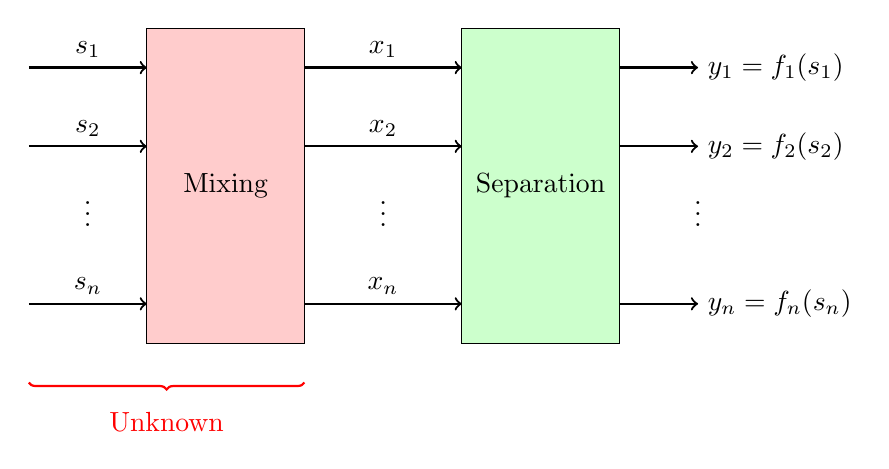
\begin{tikzpicture}

\onslide<1->{
\filldraw[draw = black, fill = red!20!white] (0,0) rectangle (2,4);
\node (text) at (1,2){Mixing};

\foreach \x in {0.5, 2.5, 3.5}
{
	\draw[->, thick] (-1.5, \x) -- (0, \x);
}

\node (vdotsin) at (-0.75,1.75){$\vdots$};


\node [anchor=south] (vdotsin) at (-0.75,0.5){$s_n$};
\node [anchor=south] (vdotsin) at (-0.75,2.5){$s_2$};
\node [anchor=south] (vdotsin) at (-0.75,3.5){$s_1$};


\foreach \x in {0.5, 2.5, 3.5}
{
	\draw[->, thick] (2, \x) -- (4, \x);
}

\node (vdotsin) at (3,1.75){$\vdots$};

\node [anchor=south] (vdotsin) at (3, 0.5){$x_n$};
\node [anchor=south] (vdotsin) at (3, 2.5){$x_2$};
\node [anchor=south] (vdotsin) at (3, 3.5){$x_1$};
}
\onslide<2->{
\filldraw[draw = black, fill = green!20!white] (4,0) rectangle (6,4);
\node (text) at (5,2){Separation};

\foreach \x in {0.5, 2.5, 3.5}
{
	\draw[->, thick] (6, \x) -- (7, \x);
}
\node (vdotsin) at (7,1.75){$\vdots$};

\node [anchor=west] (vdotsin) at (7, 0.5){$y_n = f_n(s_n)$};
\node [anchor=west] (vdotsin) at (7, 2.5){$y_2 = f_2(s_2)$};
\node [anchor=west] (vdotsin) at (7, 3.5){$y_1 = f_1(s_1)$};
}
\onslide <2->{
\draw [
red, thick,
decoration={
	brace,
	mirror,
	raise=0.5cm
},
decorate
] (-1.5, 0) -- (2, 0);

\node [red, anchor=north] at (0.25, -0.75){Unknown};

}
\end{tikzpicture}
\end{figure}
\end{frame}


\begin{frame}
\frametitle{Linear and Non-Linear BSS}
\begin{alertblock}{Darmois-Skitovic Theorem \small{[Darmois-Skitovich ∼1950]}}
In the linear setting, the model is identifiable if the sources are \textbf{non-Gaussian} random variables.
\end{alertblock}
\pause
\begin{exampleblock}{Non-Linear Mixtures}
Non-linear mixtures are harder!
\small{
\begin{equation*}
\begin{cases}

S_1 = \mathrm{Rayleigh}(\sigma)\\
S_2 = \mathrm{Uniform} [0, 2\pi]
\end{cases}
\implies
X_1 = S_1 \cos (S_2) \perp \!\!\! \perp X_2 =  S_1 \sin (S_2)
\end{equation*}
}
\end{exampleblock}
\end{frame}
\normalsize


\begin{frame}
\frametitle{Separation of Stochastic Processes (SP)}

\begin{alertblock}{Conjecture}
Let $f: \mathbb{R}^n \to \mathbb{R}^n$ be an invertible smooth mapping and $\mathbf{s}(t) \in \mathbb{R}^n$ be a vector of independent SPs. If $\mathbf{x}(t) = f(\mathbf{s}(t))$ is a vector of independent SPs, then $f$ is Affine.
\end{alertblock}
\pause

\begin{block}{Counterexample}
	\begin{itemize}
	\item Functions:
	\vspace{0.1cm}	
	
		$ f\big([s_1, s_2]^\top\big)= 
	\begin{bmatrix}
	s_1\\
	\mathrm{sign}(s_1s_2)
	\end{bmatrix}
	$
	
	\item  Stochastic Processes:
	\vspace{0.2cm}
	
	$
	\begin{cases}
	s_1[i] = s_1[i-1] + \mathcal{N}(0,1)\\
	s_2[i] = s_2[i-1] + \mathcal{N}(0,1)
	\end{cases}
	$
	\end{itemize}

\end{block}
\end{frame}


\begin{frame}
\frametitle{Proposed Algorithm}
\begin{itemize}
	
	\item  Mutual information minimization similar to the method proposed in {\small [Babaie-Zadeh et al., SP 2005]}. \\
	
	\item
	Simulation on a 2D bilinear mixture.
	
	\begin{figure}
		\centering
		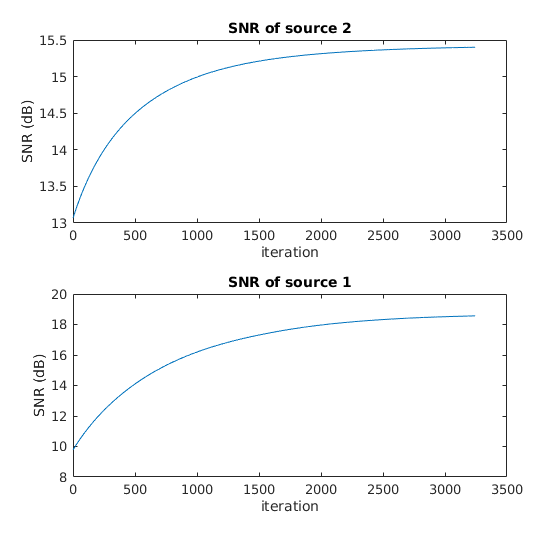
\includegraphics[scale=0.4]{./Figures/snr.png}
	\end{figure}
	
\end{itemize}
\end{frame}

\section{Noise-Contrastive Learning}
\framecard{\LARGE Noise-Contrastive Estimation (NCE)}

\begin{frame}
\frametitle{Noise-Contrastive Estimation (NCE)}

Let $\{ P_{\boldsymbol{\theta}}: \boldsymbol{\theta} \in \boldsymbol{\Theta}\}$ be a parametric family of distributions.
%\begin{itemize}
%\item \textbf{Problem: } Density estimation given $n$ i.i.d. samples %$X_1, X_2, \dots, X_n \sim P(.; \boldsymbol{\theta^*})$.
%\pause
%\item \textbf{Idea: }Use a supervised learning approach!
%\end{itemize}

\begin{columns}
	\begin{column}{0.6\textwidth}
		\begin{itemize}
			{\small
			\item Data: $X_1, X_2, \dots, X_n \sim P(,;\boldsymbol{\theta^*})$
			\item Noise: $Y_1, Y_2, \dots, Y_n \sim P_n $}

		
		\end{itemize}
	\end{column}
	\begin{column}{0.4\textwidth}  %%<--- here
		\begin{center}
			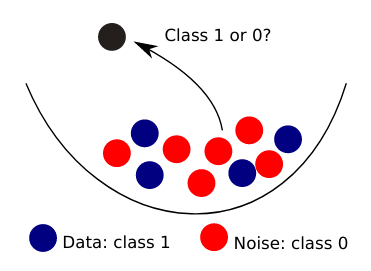
\includegraphics[width=\textwidth]{./Figures/class.png}
		\end{center}
	\end{column}			
\end{columns}
\vspace{0.5cm}
$$\Big\{\overbrace{(\mathbf{x}_1, 0),(\mathbf{x}_2, 0), \dots, (\mathbf{x}_n, 0)}^{P(., \boldsymbol{\theta^*})}, \overbrace{(\mathbf{y}_1, 1), (\mathbf{y}_2, 1), \dots, (\mathbf{y}_n,1)}^{P_n}\Big\}$$
\end{frame}

\begin{frame}

\begin{itemize}
\item {\bf Model}: \hspace{0.5cm}
$P(C=1 | \mathbf{u}, \boldsymbol{\theta}) = \frac{1}{1 + G(\mathbf{u}, \boldsymbol{\theta})}, \;\;\; G(\mathbf{u}, \boldsymbol{\theta}) \geq 0$
\vspace{0.5cm}


\item {\bf Conditional Liklihood}:
$$J_n^{\mathrm{NCE}}(\boldsymbol{\theta}) = \frac{1}{n} \Big(
\sum_{i = 1}^{n} \log P(C = 1| \mathbf{x}_i; \boldsymbol{\theta})
+
\sum_{i = 1}^{n} \log P(C = 0| \mathbf{y}_i; \boldsymbol{\theta})
\Big)$$


\item {\bf Learning Algorithm}: $\hat{\boldsymbol{\theta}}_n = \mathrm{argmax}\; J_n^{\mathrm{NCE}}(\boldsymbol{\theta})$

\end{itemize}

\begin{alertblock}{Consistency  {\scriptsize[Gutmann \& Hyvarinen, JMLR 2010]}}
	Asymptotically as $n \to \infty$: 
	$G(\mathbf{u}, \hat{\boldsymbol{\theta}}_n) \asto \frac{P(\mathbf{u}, \boldsymbol{\theta^*})}{P_n(\mathbf{u})} $
\end{alertblock}

\end{frame}


\begin{frame}
\frametitle{Time-Contrastive Learning}
\begin{columns}
	\begin{column}{0.5\textwidth}
		\begin{figure}
			\centering
			{\bf\scriptsize Time-Contrastive Learning}\\
			\scriptsize{[Hyvarinen et al., NIPS 2016]}
			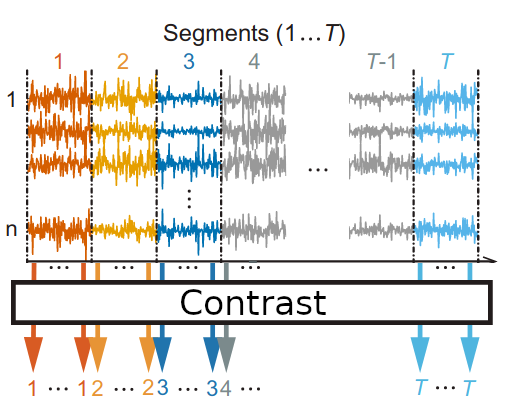
\includegraphics[scale=0.3]{./Figures/t.png}
		\end{figure}
	\end{column}
	\begin{column}{0.5\textwidth}  %%<--- here
			{\small
		
			$$\log p_\tau(s_i)= \lambda_{i}(\tau) q(s_i) + C$$\\
				
			$$\log p_\tau(s_i)=   \sum_{v=1}^V \lambda_{i,v}(\tau) q_{i,v}(s_i) + C.$$}
	\end{column}
\end{columns}
\end{frame}



\section{Gaussanity-based Methods}
\framecard{\LARGE Gaussanity-based Methods}

\begin{frame}
\frametitle{Polynomial Mappings}

\begin{alertblock}{Polynomial Mixing Theorem}
Only linear polynomials can transform a Gaussian vector to a Gaussian vector.
\end{alertblock}

\begin{figure}
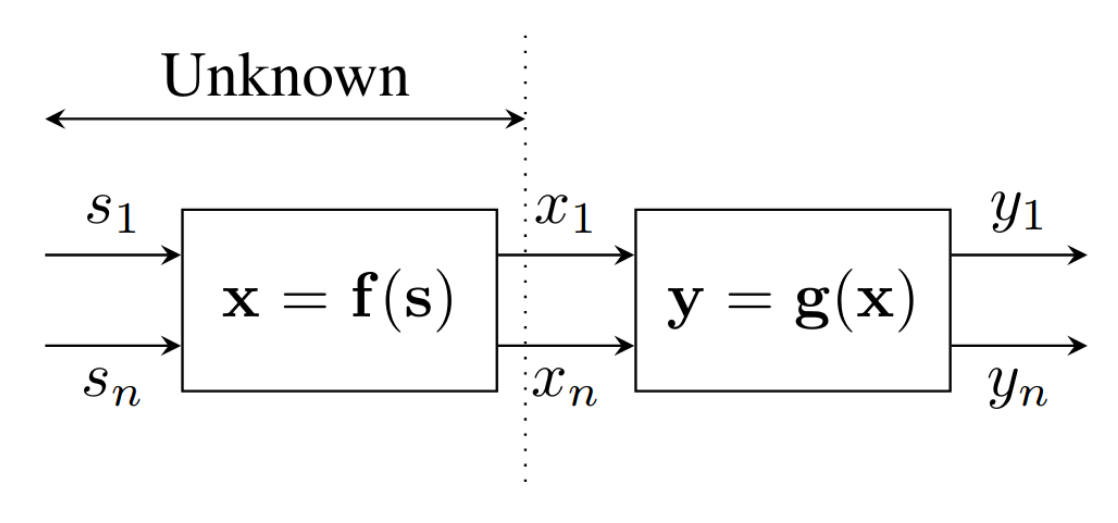
\includegraphics[scale=0.17]{./Figures/mixdemix.png}
\end{figure}

\end{frame}


\begin{frame}
\frametitle{Separation Algorithm}
\begin{itemize}
\item A parametric model for the separating polynomial:
{\small\begin{equation*}
\label{E_Parametrizing}
{\bf g}({\bf x})=
\begin{bmatrix}
g_1({\bf x}) \\
g_2({\bf x}) \\
\vdots \\
g_n({\bf x})
\end{bmatrix}=
\begin{bmatrix}
\theta_{11} & \theta_{12} & \dots & \theta_{1s} \\
\theta_{21} & \theta_{22} & \dots & \theta_{1s} \\
\vdots&\vdots&\ddots&\vdots \\
\theta_{n1} & \theta_{n2} & \dots & \theta_{ns}
\end{bmatrix}
\begin{bmatrix}
x_1\\
x_1x_2\\
x_1x_2x_3\\
\vdots\\
x_k^p
\end{bmatrix}
=
\boldsymbol{\Theta}{\bf k}({\bf x})
\end{equation*}}
\vspace{-0.5cm}
\item Measures of non-Gaussanity:

\begin{itemize}
	\item Negative Entropy: 
	\hspace{0.35cm}	
	$
	\boldsymbol{\mathcal{J}_1}({ y_i})=\boldsymbol{H}({ \tilde{y}_i})-\boldsymbol{H}({ y_i})
	$
	\vspace{0.2cm}
	
	\item Difference of CDFs:\hspace{0.3cm}
	$
	\boldsymbol{\mathcal{J}_2}({ x_i})=\sup_x |\Phi(x) - \hat{F}(x)|
	$
	\item Kurtosis:\hspace{1.9cm}
	$
	\boldsymbol{\mathcal{J}_3}({ x_i})=\Big[\hat{\mathbb{E}}[X^4] - 3(\hat{\mathbb{E}}[X^2])^2 \Big]^2
	$
\end{itemize}



\item Optimization problem:
\begin{equation*}
\underset{\boldsymbol{\Theta}}{\min} \ \| \boldsymbol{\mathcal{J}}(\boldsymbol{\Theta}{\bf k}({\bf x})) \|_2^2
\end{equation*}

\end{itemize}
\end{frame}


\begin{frame}
\frametitle{Simulations}
\small
Let $s_1, s_2 \sim \mathcal{N}(0,1)$ and $s_1 \bigCI s_2$.

\begin{equation*}
\label{E_SimulationMixture}
\begin{bmatrix}
s_1 \\
s_2
\end{bmatrix}
\rightarrow
\begin{bmatrix}
x_1 \\
x_2
\end{bmatrix}
=
\begin{bmatrix}
s_1+(s_1+s_2)^3 \\
s_2-(s_1+s_2)^3
\end{bmatrix}
\end{equation*}

\normalsize
\begin{columns}
		\begin{column}{0.33\textwidth}  %%<--- here
		\begin{center}
			Negative Entropy
			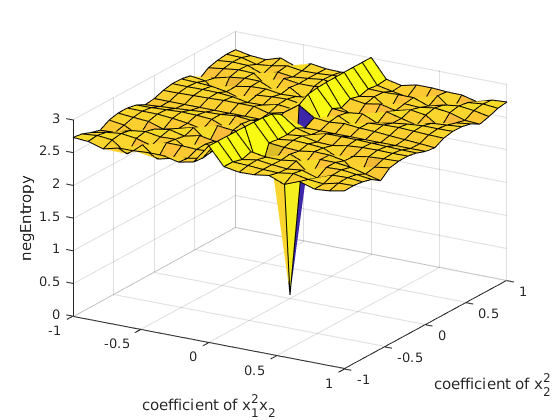
\includegraphics[width=\textwidth]{./Figures/negent.png}
		\end{center}
	\end{column}	
	\begin{column}{0.33\textwidth}  %%<--- here
		\begin{center}
			Difference of CDFs
			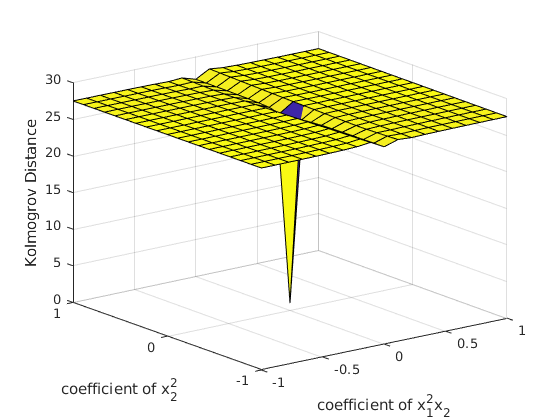
\includegraphics[width=\textwidth]{./Figures/kolmo.png}
		\end{center}
	\end{column}	
	\begin{column}{0.33\textwidth}  %%<--- here
		\begin{center}
			Kurtosis
			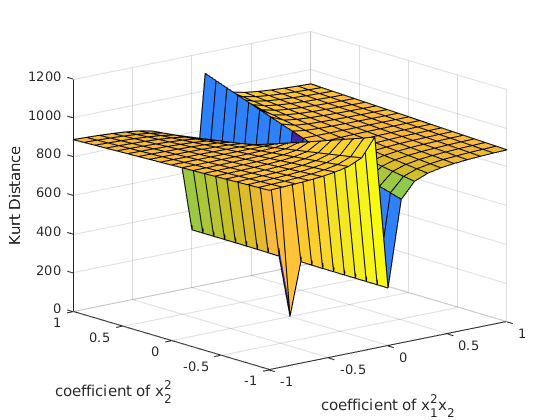
\includegraphics[width=\textwidth]{./Figures/kurt.png}
		\end{center}
	\end{column}			
\end{columns}
\end{frame}

\begin{frame}
	\frametitle{Negative Entropy}	
	\centering
	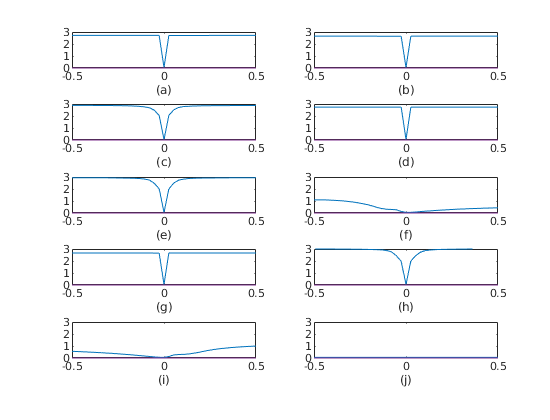
\includegraphics[width=0.8\textwidth]{./Figures/negent1.png}
\end{frame}

\begin{frame}
	\frametitle{Difference of CDFs}
	\centering
	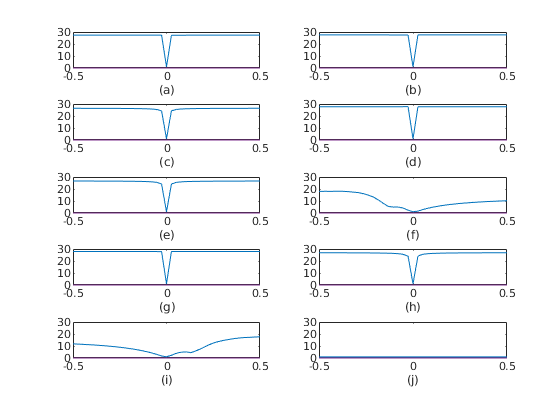
\includegraphics[width=0.8\textwidth]{./Figures/kolmo1.png}
\end{frame}

\begin{frame}
	\frametitle{Kurtosis}
	\centering
	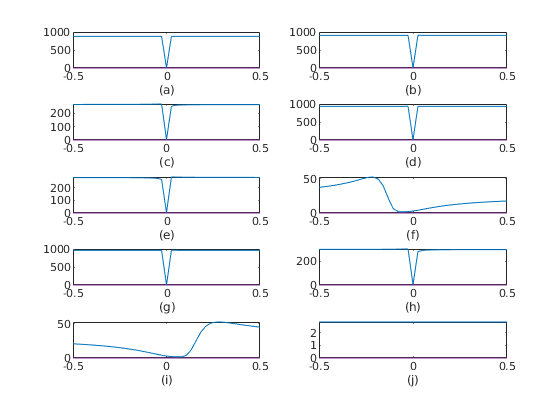
\includegraphics[width=0.8\textwidth]{./Figures/kurt1.png}
\end{frame}
\section{Another Idea!}
\framecard{\LARGE Another Idea}

\begin{frame}
\frametitle{Monotonicity of Mixtures}
We have proved the following theorem:

\begin{block}{Monotone functions do not preserve Gaussanity!}
Let ${\bf f} = (f_1, f_2, \dots, f_n)^\top: \mathbb{R}^n \to \mathbb{R}^n$ be a continuous and invertible mixing system and all $f_i$s be monotone functions with respect to all of their inputs. If ${\bf f}$ preserves Gaussanity, then ${\bf f}$ is Affine.
\end{block}

\pause
Connections to BSS:
\begin{itemize}
	\item Not that obvious. Mixing and Demixing?
	\pause
	\item How about subsets of monotone functions?
\end{itemize}



\end{frame}

\framecard{Thank You.}

\begin{frame}
\begin{figure}
	\centering
	{\bf\scriptsize Permutation-Contrastive Learning}\\
	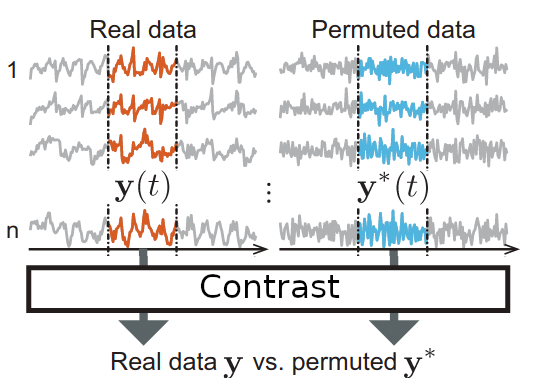
\includegraphics[scale=0.3]{./Figures/tt.png}
\end{figure}		
{\small
	The proof is flawed, but can be fixed with a re-sampling trick.}
\end{frame}

\begin{frame}
\frametitle{Permutation Contrastive Learning}	
\begin{alertblock}{Permutation Contrastive Separation \scriptsize{[Hyvarinen et al., NIPS 2016]}}	
	The mixture
	$\textbf{x}(t) = \textbf{f}\big(\textbf{s}(t)\big)$ is separable if:
	\begin{itemize}
		\item
		$\textbf{f}$ is invertible and smooth!
		\item
		$s_i(t)$:  \textbf{stationary},  \textbf{ergodic} and  \textbf{ \textit{uniformly dependent}}.
		\item
		$s_i(t)$ are not \textbf{ \textit{quasi-Gaussian}}.		
	\end{itemize}
\end{alertblock}

\begin{block}{Contribution}
	The proof presented in {\small [Hyvarinen et al., NIPS 2016]} is flawed and assumes that the time shuffled SP is independent in time. This error can be fixed by a re-sampling trick.
\end{block}
\end{frame}



\end{document}


\begin{frame}
\frametitle{Permutation Contrastive Learning}	
\begin{alertblock}{Permutation Contrastive Separation \scriptsize{[Hyvarinen et al., NIPS 2016]}}	
	The mixture
	$\textbf{x}(t) = \textbf{f}\big(\textbf{s}(t)\big)$ is separable if:
	\begin{itemize}
		\item
		$\textbf{f}$ is invertible and smooth!
		\item
		$s_i(t)$:  \textbf{stationary},  \textbf{ergodic} and  \textbf{ \textit{uniformly dependent}}.
		\item
		$s_i(t)$ are not \textbf{ \textit{quasi-Gaussian}}.		
	\end{itemize}
\end{alertblock}

\begin{block}{Contribution}
	The proof presented in {\small [Hyvarinen et al., NIPS 2016]} is flawed and assumes that the time shuffled SP is independent in time. This error can be fixed by a re-sampling trick.
\end{block}
\end{frame}
\begin{frame}
\frametitle{Time-Contrastive Learning}
\begin{alertblock}{Time Contrastive Learning \scriptsize{[Hyvarinen et al., NIPS 2016]}}	
	The smooth mixture
	$\textbf{x}(t) = \textbf{f}\big(\textbf{s}(t)\big)$ is separable if 
	\vspace{-0.1cm}
	$$\log p_\tau(s_i)= \lambda_{i}(\tau) q(s_i) + C$$		
	plus some technical conditions on $\lambda_i$.
\end{alertblock}

\begin{block}{Generalization}
	We have generalized the theorem above for 
	\vspace{-0.4cm}
	$$\log p_\tau(s_i)=   \sum_{v=1}^V \lambda_{i,v}(\tau) q_{i,v}(s_i) + C.$$
	\vspace{-0.4cm}
\end{block}

\vspace{0.3cm}
\vspace{-1cm}
\begin{figure}
	\centering
	{\bf\scriptsize Permutation-Contrastive Learning}
	\scriptsize{[Hyvarinen et al., AISTAT 2017]}
	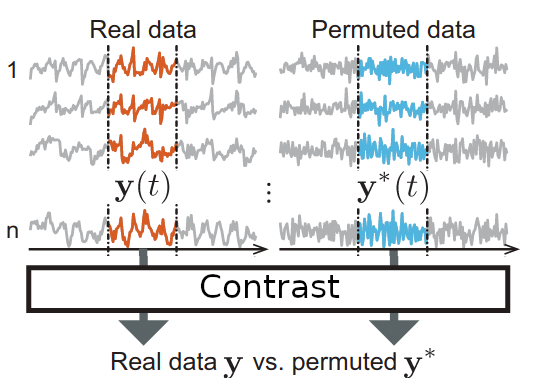
\includegraphics[scale=0.3]{./Figures/tt.png}
\end{figure}		
{\small
	The proof is flawed, but can be fixed with a re-sampling trick.}
\end{frame}

